\documentclass{beamer}
\usepackage{amsmath}
\usepackage[english]{babel} %set language; note: after changing this, you need to delete all auxiliary files to recompile
\usepackage[utf8]{inputenc} %define file encoding; latin1 is the other often used option
\usepackage{csquotes} % provides context sensitive quotation facilities
\usepackage{graphicx} %allows for inserting figures
\usepackage{booktabs} % for table formatting without vertical lines
\usepackage{textcomp} % allow for example using the Euro sign with \texteuro
\usepackage{stackengine}
\usepackage{wasysym}
\usepackage{tikzsymbols}
\usepackage{textcomp}
\usepackage{xcolor}
\usepackage[dvipsnames]{xcolor}
\usepackage{colortbl}
\usepackage{adjustbox}
\usepackage{tikz} % allows drawing figures
\usetikzlibrary{decorations.pathreplacing}
\newcommand{\bubblethis}[2]{
        \tikz[remember picture,baseline]{\node[anchor=base,inner sep=0,outer sep=0]%
        (#1) {\underline{#1}};\node[overlay,cloud callout,callout relative pointer={(0.2cm,-0.7cm)},%
        aspect=2.5,fill=yellow!90] at ($(#1.north)+(-0.5cm,1.6cm)$) {#2};}%
    }%
\tikzset{face/.style={shape=circle,minimum size=4ex,shading=radial,outer sep=0pt,
        inner color=white!50!yellow,outer color= yellow!70!orange}}
%% Some commands to make the code easier
\newcommand{\emoticon}[1][]{%
  \node[face,#1] (emoticon) {};
  %% The eyes are fixed.
  \draw[fill=white] (-1ex,0ex) ..controls (-0.5ex,0.2ex)and(0.5ex,0.2ex)..
        (1ex,0.0ex) ..controls ( 1.5ex,1.5ex)and( 0.2ex,1.7ex)..
        (0ex,0.4ex) ..controls (-0.2ex,1.7ex)and(-1.5ex,1.5ex)..
        (-1ex,0ex)--cycle;}
\newcommand{\pupils}{
  %% standard pupils
  \fill[shift={(0.5ex,0.5ex)},rotate=80] 
       (0,0) ellipse (0.3ex and 0.15ex);
  \fill[shift={(-0.5ex,0.5ex)},rotate=100] 
       (0,0) ellipse (0.3ex and 0.15ex);}

\newcommand{\emoticonname}[1]{
  \node[below=1ex of emoticon,font=\footnotesize,
        minimum width=4cm]{#1};}
\usepackage{scalerel}
\usetikzlibrary{positioning}
\usepackage{xcolor,amssymb}
\newcommand\dangersignb[1][2ex]{%
  \scaleto{\stackengine{0.3pt}{\scalebox{1.1}[.9]{%
  \color{red}$\blacktriangle$}}{\tiny\bfseries !}{O}{c}{F}{F}{L}}{#1}%
}
\newcommand\dangersignw[1][2ex]{%
  \scaleto{\stackengine{0.3pt}{\scalebox{1.1}[.9]{%
  \color{red}$\blacktriangle$}}{\color{white}\tiny\bfseries !}{O}{c}{F}{F}{L}}{#1}%
}
\usepackage{fontawesome} % Social Icons
\usepackage{epstopdf} % allow embedding eps-figures
\usepackage{tikz} % allows drawing figures
\usepackage{amsmath,amssymb,amsthm} %advanced math facilities
\usepackage{lmodern} %uses font that support italic and bold at the same time
\usepackage{hyperref}
\usepackage{tikz}
\hypersetup{
    colorlinks=true,
    linkcolor=blue,
    filecolor=magenta,      
    urlcolor=blue,
}
\usepackage{tcolorbox}
%add citation management using BibLaTeX
\usepackage[citestyle=authoryear-comp, %define style for citations
    bibstyle=authoryear-comp, %define style for bibliography
    maxbibnames=10, %maximum number of authors displayed in bibliography
    minbibnames=1, %minimum number of authors displayed in bibliography
    maxcitenames=3, %maximum number of authors displayed in citations before using et al.
    minnames=1, %maximum number of authors displayed in citations before using et al.
    datezeros=false, % do not print dates with leading zeros
    date=long, %use long formats for dates
    isbn=false,% show no ISBNs in bibliography (applies only if not a mandatory field)
    url=false,% show no urls in bibliography (applies only if not a mandatory field)
    doi=false, % show no dois in bibliography (applies only if not a mandatory field)
    eprint=false, %show no eprint-field in bibliography (applies only if not a mandatory field)
    backend=biber %use biber as the backend; backend=bibtex is less powerful, but easier to install
    ]{biblatex}
\addbibresource{../mybibfile.bib} %define bib-file located one folder higher


\usefonttheme[onlymath]{serif} %set math font to serif ones

\definecolor{beamerblue}{rgb}{0.2,0.2,0.7} %define beamerblue color for later use

%%% defines highlight command to set text blue
\newcommand{\highlight}[1]{{\color{blue}{#1}}}


%%%%%%% commands defining backup slides so that frame numbering is correct

\newcommand{\backupbegin}{
   \newcounter{framenumberappendix}
   \setcounter{framenumberappendix}{\value{framenumber}}
}
\newcommand{\backupend}{
   \addtocounter{framenumberappendix}{-\value{framenumber}}
   \addtocounter{framenumber}{\value{framenumberappendix}}
}

%%%% end of defining backup slides

%Specify figure caption, see also http://tex.stackexchange.com/questions/155738/caption-package-not-working-with-beamer
\setbeamertemplate{caption}{\insertcaption} %redefines caption to remove label "Figure".
%\setbeamerfont{caption}{size=\scriptsize,shape=\itshape,series=\bfseries} %sets figure  caption bold and italic and makes it smaller

\newtcolorbox{boxA}{
    fontupper = \bf,
    boxrule = 1.5pt,
    colframe = black % frame color
}
\newtcolorbox{boxB}{
    boxrule = 1.5pt,
    colframe = blue!70!black,, % frame color
    colback = blue!7!white,
}
\usetheme{Boadilla}

% --------------------
% Overall information
% --------------------
\title[Economía I]{Economía I \vspace{4mm}
\\ Magistral 23: Mercado de dinero}
\date{}
\author[Franco Riottini]{Franco Riottini}
\vspace{0.4cm}
\institute[]{Universidad de San Andrés} 


\begin{document}

\begin{frame}
\titlepage
\centering

\includegraphics[scale=0.2]{../Figures/logoUDESA.jpg} 
\end{frame}

\begin{frame}{Tipos de dinero}
    \begin{itemize}
        \item Durante la mayor parte de la historia de la humanidad se utilizó dinero mercancía (commodity money)
            \begin{itemize}
                \item Mercancías con valor intrínseco que se usaban para comerciar: Oro, plata, sal, cigarrillos, etc.
            \end{itemize}
        \item Hoy en día, casi todo el dinero es fiduciario (fiat money)               
        \begin{itemize}
            \item Sin valor intrínseco, pero que se utiliza porque el gobierno lo hace de curso legal: Pesos, euros, dólares, bonos provinciales (cuasimonedas), etc.
            \item Ahora es casi natural, pero tomó mucho tiempo: Problemas de confianza, falsificación, funcionamiento, etc.
        \end{itemize}
    \end{itemize}
\end{frame}

\begin{frame}{Commodity money}
            \begin{figure} [H]   
  \centering
  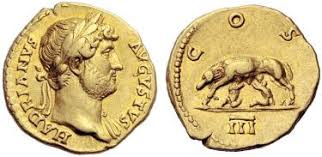
\includegraphics[width=.8\textwidth]{../Figures/C32.1.jpg}
      \caption{Monedas carcomidas}
\end{figure}
\end{frame}

\begin{frame}{Dinero Papel}
    \begin{itemize}
        \item Comienza a usarse en China en el Siglo VII
        \item Antes de los bancos centrales los emitían los bancos 
    \end{itemize}
\begin{figure} [H]   
    \centering
    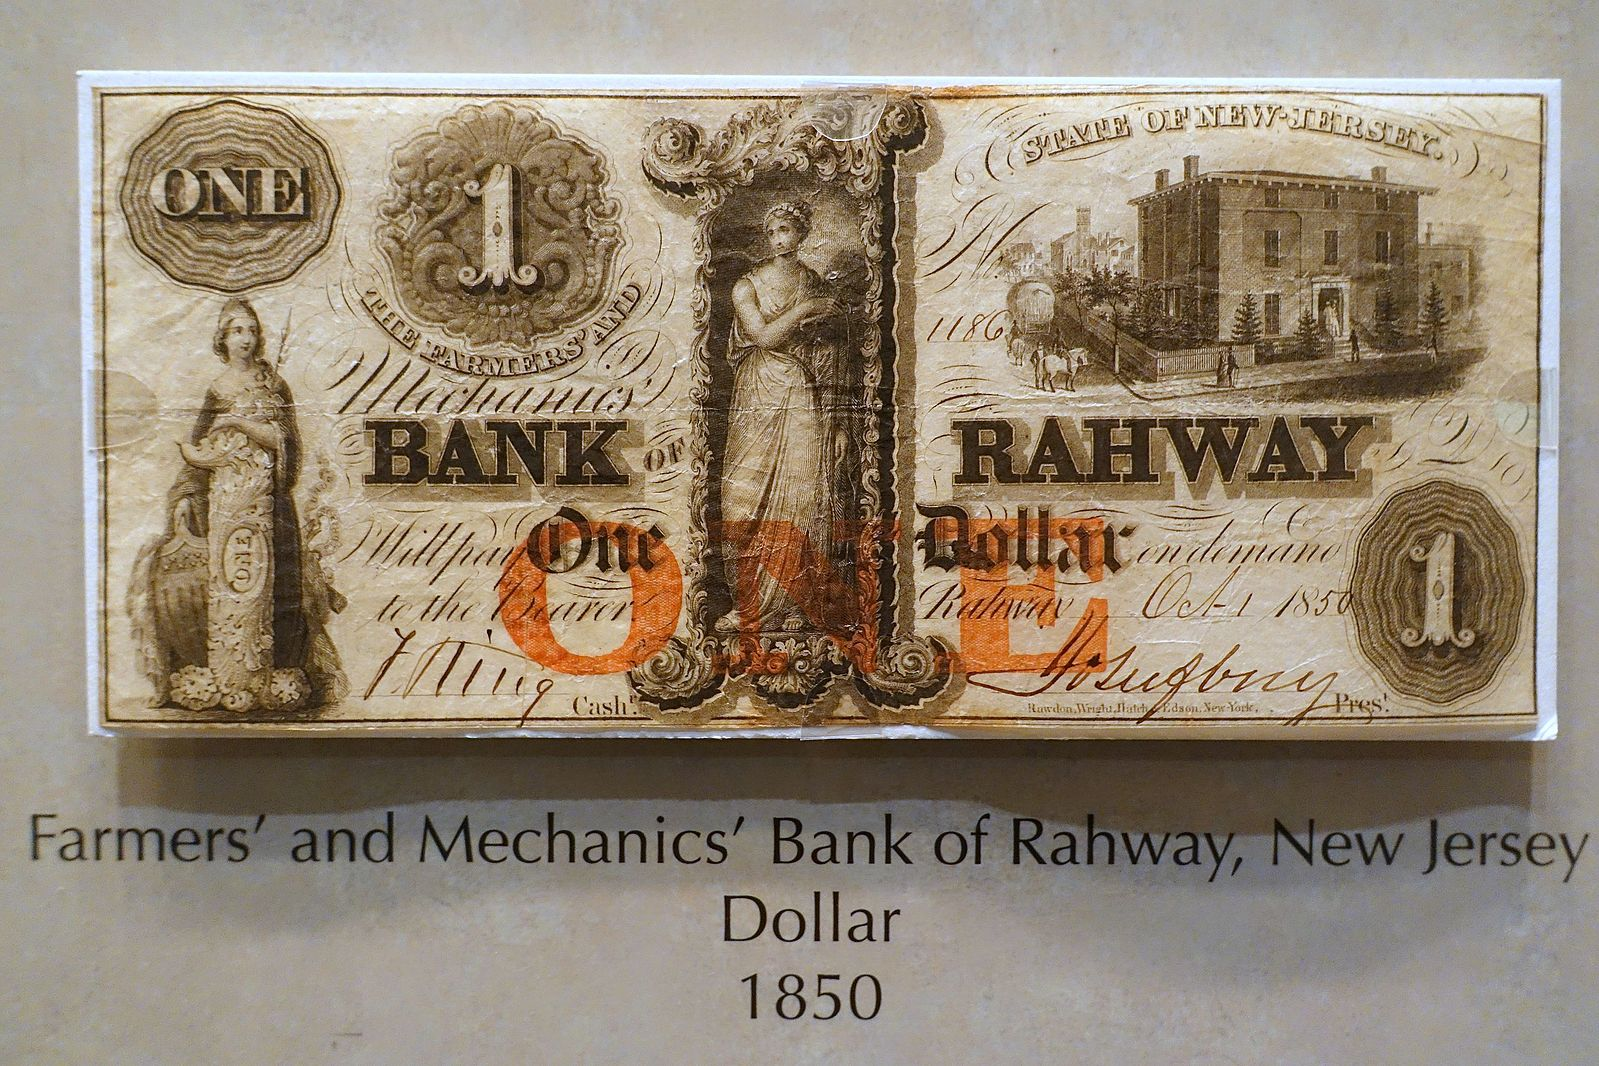
\includegraphics[width=.35\textwidth]{../Figures/C32.2.jpg}
    \caption{Dollar de Bank of Rahway, New Jersey, 1850. Via Wikimedia Commons}
\end{figure}

\begin{figure} [H]   
    \centering
    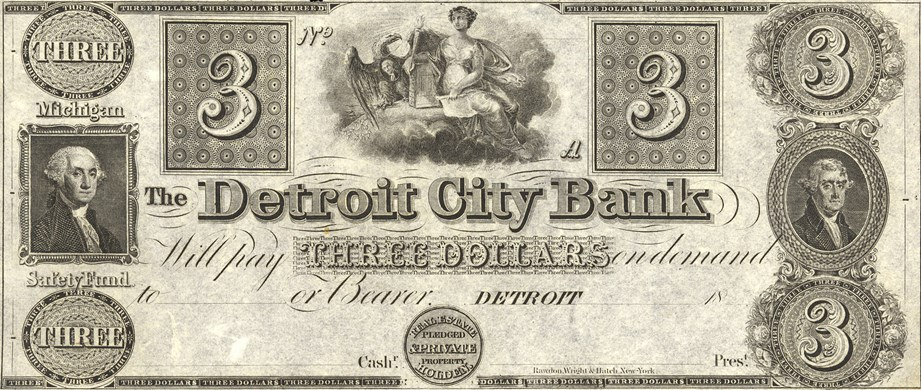
\includegraphics[width=.35\textwidth]{../Figures/C32.3.jpeg}
    \caption{Detroit City Bank \$3 Note}
\end{figure}

\end{frame}
        
\begin{frame}{El dinero}
    \begin{figure} [H]   
    \centering
        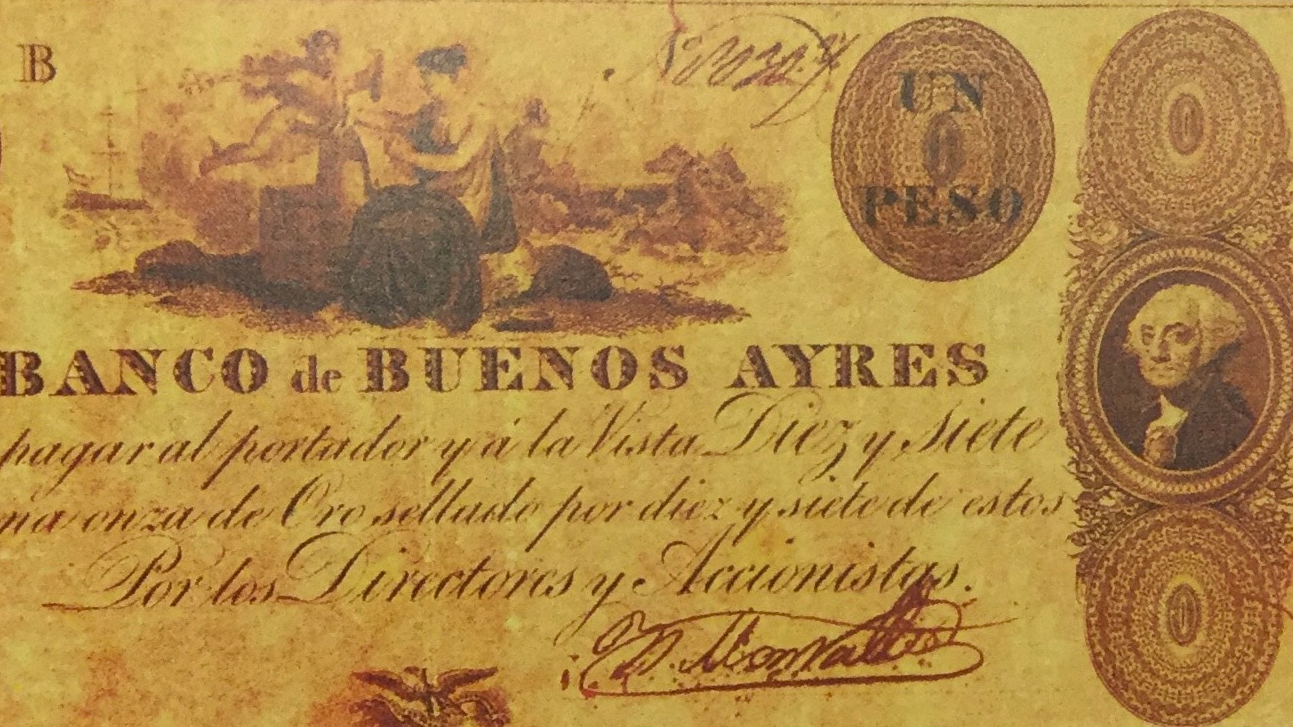
\includegraphics[width=.35\textwidth]{../Figures/C32.4.jpg}
        \caption{Billetes emitidos por el Banco Provincia de Buenos Aires}
    \end{figure}
    \begin{figure} [H]   
        \centering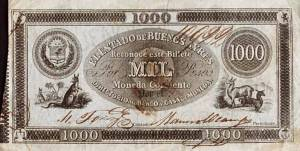
\includegraphics[width=.35\textwidth]{../Figures/C32.5.jpg}
        \caption{Billetes emitidos por el Banco Provincia de Buenos Aires}
    \end{figure}
    \begin{itemize}
        \item Luego lo monopolizaron los bancos centrales
        \item Y hoy volvemos a la multiplicidad de monedas 
    \end{itemize}     
\end{frame}

\begin{frame}{Funciones del dinero}
    \small
    \begin{center}
    \begin{tabular}{@{}p{0.27\textwidth} p{0.5\textwidth} p{0.17\textwidth}@{}}
    \toprule
    \textbf{Función} & \textbf{Definición operativa} & \textbf{Fragilidad principal} \\
    \midrule
    \textbf{\alert{Medio de cambio}} & Instrumento aceptado para cancelar transacciones & Confianza \\
    \textbf{\alert{Unidad de cuenta}} & Patrón numérico para fijar precios y registrar deudas & Inflación \\
    \textbf{\alert{Depósito de valor}} & Vehículo que permite transferir poder de compra al futuro & Inflación \\
    \bottomrule
    \end{tabular}
    \end{center}
    \small
    \begin{boxA}
        \centering
        ¿Cuánta liquidez desea la economía y quién la provee?
    \end{boxA}
\end{frame}


\begin{frame}{La demanda de dinero}
    \begin{itemize}
        \item La demanda de dinero es lo que la gente demanda de dinero, es cuánto dinero desea tener la sociedad
        \item Se explica por dos motivos principalmente: por motivo \textbf{transaccional} y por motivo \textbf{especulativo}
        \begin{itemize}
        \item Por transacciones $\Rightarrow P*Y \Rightarrow$ a mayores precios o mayor nivel de actividad aumenta la demanda de dinero por transacciones
        \item Costo de oportunidad $\Rightarrow i \Rightarrow $ la demanda de dinero depende negativamente de la tasa de interés que es el costo de oportunidad del dinero
    \end{itemize}
    \item La llegada de las tarjetas de crédito, el dinero bancario y la agilidad de transferir dinero de activos líquidos a dinero, entre otros, son elementos que han ido cambiando drásticamente la demanda de dinero en el tiempo
    \item La demanda de dinero puede referirse a distintas ‘clases’ de dinero, según el nivel de liquidez que consideramos relevante.
    \end{itemize}
\end{frame}

\begin{frame}{La oferta de dinero y los agregados monetarios}
    \small
    \begin{block}{\textbf{¿Qué es la oferta de dinero?}}
    \begin{itemize}
        \item No hay una única medida: depende del grado de liquidez del activo considerado.
        \item El dinero puede ser creado tanto por el Banco Central (\alert{oferta primaria}) como por los bancos comerciales (\alert{oferta secundaria}).
    \end{itemize}
    \end{block}
    \vspace{0.3em}
    \begin{center}
    \small
    \setlength{\tabcolsep}{3.5pt}
    \begin{tabular}{@{}l p{0.33\textwidth} p{0.23\textwidth}@{}}
    \toprule
    \textbf{Agregado} & \textbf{Componentes} & \textbf{Quién lo crea} \\
    \midrule
    \textbf{M0}  & Circulante + encajes bancarios         & BCRA \\
    \textbf{M1}  & Circulante + depósitos a la vista      & BCRA + bancos \\
    \textbf{M2}  & M1 + caja de ahorro                    & Bancos \\
    \textbf{M3}  & M2 + plazo fijo                        & Bancos \\
    \textbf{M\textit{n}} & M3 + otros activos líquidos        & Sistema financiero \\
    \bottomrule
    \end{tabular}
    \end{center}
    \vspace{0.5em}
    \footnotesize
    A mayor número del agregado, menor liquidez pero mayor inclusión de activos.
\end{frame}

\begin{frame}
\frametitle{¿Qué es el Banco Central?}
\begin{itemize}
    \item Un banco particular
        \begin{itemize}
            \item Es generalmente propiedad del gobierno.
            \item Actúa como banquero de los bancos comerciales: Que tienen `reservas' en el Banco Central.
            \item Es prestamista de ultima instancia.
            \item Es el único que puede crear moneda de curso legal.
        \end{itemize}
    \item Dinero en el sentido amplio
        \begin{itemize}
            \item Base monetaria (base money) o M0: Billetes y monedas, más cuentas depositadas en el Banco Central (encajes).
            \item Depósitos (bank money): Dinero creado por los bancos comerciales al extender crédito.
        \end{itemize}
\end{itemize}
\end{frame}

\begin{frame}
    \begin{table}[h!]
    \centering
    \renewcommand{\arraystretch}{1.3}
    \setlength{\tabcolsep}{8pt}
    \begin{tabular}{>{\columncolor{yellow!70}}c|>{\columncolor{yellow!40}}c}
    \multicolumn{2}{c}{\cellcolor{yellow!90}\textbf{Banco Central}} \\
    \textbf{Activo} & \textbf{Pasivo} \\
    \hline
    \textbf{Reservas Internacionales} & 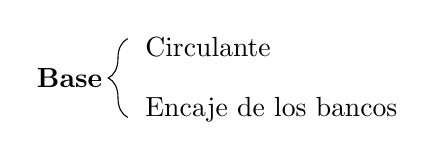
\begin{tikzpicture}
                % Texto "Base"
                \node[anchor=east] (base) at (0,0) {\textbf{Base}};
                % Llave (brace)
                \draw [decorate,decoration={brace,amplitude=7pt}] (0.2,-0.5) -- (0.2,0.5);
                % Elementos agrupados
                \node[anchor=west] at (0.3,0.4) {Circulante};
                \node[anchor=west] at (0.3,-0.4) {Encaje de los bancos};
                \end{tikzpicture} \\
    \textbf{Crédito doméstico} & \textbf{Pasivos remunerados} \\
    \end{tabular}
    \end{table}
\end{frame}

\begin{frame}{¿Qué más hace el Banco Central?}
    \begin{itemize}
        \item Crea y regula la cantidad de dinero en la economía
        \item Regula la actividad bancaria
        \item Es prestamista de última instancia
        \item Maneja la política cambiaria 
    \end{itemize}
\end{frame}

\begin{frame}
\frametitle{¿Qué son los bancos?}
\begin{itemize}
    \item Son intermediarios financieros
    \item Instituciones que reciben fondos de personas y empresas, y los utilizan para comprar bonos o acciones, o para hacer préstamos a otros agentes
    \begin{itemize}
        \item Los bancos piden prestado a los hogares (depósitos), otros bancos, y el banco central \\
        \item El interés que pagan por los depósitos (tasa de interés pasiva) es menor que el que cobran en préstamos (tasa de interés activa, lending rate), y así obtienen beneficios:
        \[ \text{Spread} = \text{Interés activo} - \text{Interés pasivo} \]
    \end{itemize}
\end{itemize}
\end{frame}

\begin{frame}{Riesgos que tienen que manejar los bancos}
    \begin{itemize}
        \item \textbf{Riesgo de credito o default}: Riesgo de que los créditos del banco no sean repagados
        \item \textbf{Riesgo de madurez}: Riesgo de que los activos y pasivos del banco no tengan la misma duración
        \item \textbf{Riesgo de liquidez}: Riesgo de que el activo no se pueda transformar en efectivo (liquidar) sin generar una pérdida financiera
    \end{itemize}
    Estos riesgos pueden hacer que los depositantes no tomen las decisiones más correctas, lo que puede generar riesgos sistémicos. El banco central ayuda a mitigar este riesgo (principalmente de \textit{corridas}) obligando a los bancos a guardar un porcentaje de los depósitos (encajes). 
\end{frame}


\begin{frame}{El multiplicador monetario}
    \begin{itemize}
        \item Los bancos comerciales también crean dinero.
        \item Surge de su posibilidad de entregar créditos.
        \item La llamamos creación secundaria de dinero.
        \item Es afectado por la tasa de encajes y por la preferencia por la liquidez.
        \item Los encajes se usan para regular la cantidad de dinero
    \end{itemize}
\end{frame}

\begin{frame}{El multiplicador monetario}
\begin{itemize}
    \item[\textbullet] \textbf{Ejemplo 1:} circulante inicial = 100, encajes = 10\%
    \begin{center}
        \scriptsize
        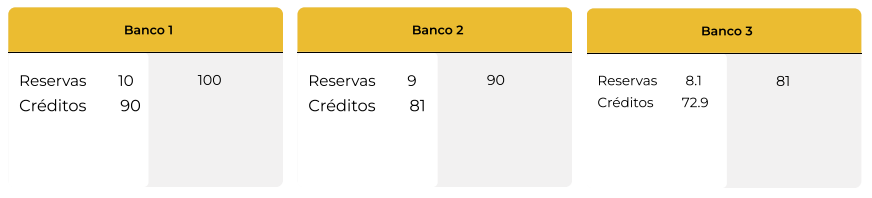
\includegraphics[width=8.5cm]{../Figures/C37.15.png}
        
        \vspace{0.3em}
        $M1 = \text{circulante} + \text{depósitos} = 100 + 90 + 81 + 72.9 + \dots = 1000$
    \end{center}

    \item[\textbullet] \textbf{Ejemplo 2:} circulante inicial = 100, encajes = 20\%
    \begin{center}
        \scriptsize
        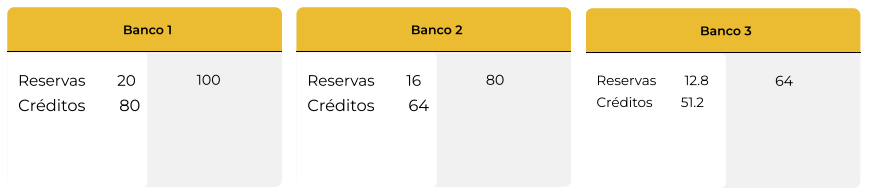
\includegraphics[width=8.5cm]{../Figures/C37.16.png}
        
        \vspace{0.3em}
        $M1 = \text{circulante} + \text{depósitos} = 100 + 80 + 64 + 51.2 + \dots = 500$
    \end{center}
\end{itemize}
\end{frame}

\begin{frame}{¿Qué pasa si el Banco Central emite más dinero?}
    \begin{boxB}
        \centering
        En las próximas clases vamos a dar un paso más y tratar de responder una pregunta clave para toda la macroeconomía:

        \vspace{0.2em}
        \textit{Si el Banco Central emite más dinero, ¿qué pasa con los precios? ¿y con el poder de compra de la gente?}
    \end{boxB}
\end{frame}


\end{document}